\documentclass[12pt, twoside]{article}
\usepackage[francais]{babel}
\usepackage[T1]{fontenc}
\usepackage[latin1]{inputenc}
\usepackage[left=6mm, right=6mm, top=6mm, bottom=3mm]{geometry}
\usepackage{float}
\usepackage{graphicx}
\usepackage{array}
\usepackage{multirow}
\usepackage{amsmath,amssymb,mathrsfs}
\usepackage{soul}
\usepackage{textcomp}
\usepackage{eurosym}
 \usepackage{variations}
\usepackage{tabvar}


\pagestyle{empty}

\begin{document}


\section*{\center{Devoir maison 2}}

\textit{Devoir � rendre sur feuille grand format petits
carreaux pour le \ul{vendredi 6 novembre 2009}.}

\enskip


\textit{Remarque: La r�daction et la justifcation des r�sultats seront pris en
compte.}

\subsection*{Exercice 1}




\begin{tabular}{cc}
\begin{minipage}{13cm}

$\mathcal{L}$ est un cercle de centre E.
\begin{enumerate}
  \item Montrer que le triangle AFD est rectangle en F.
  \item Que peut-on dire des droites (CA) et (CB)? Justifier.
\end{enumerate}

\end{minipage}
&
\begin{minipage}{5cm}
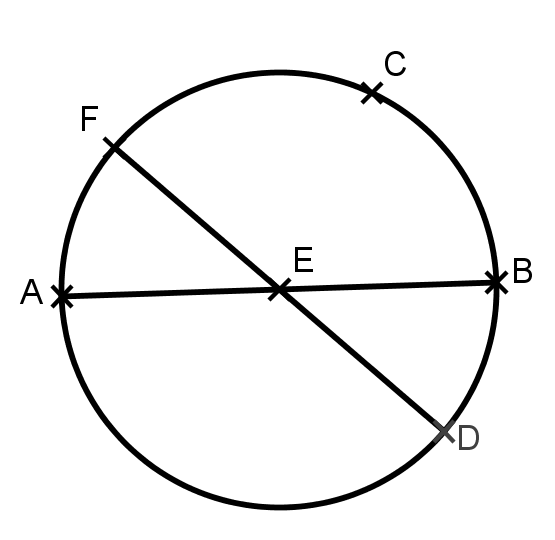
\includegraphics[width=4cm]{images/ex1.png}
\end{minipage}
\end{tabular}




\subsection*{Exercice 2}


A partir des informations port�es sur la figure suivante, d�terminer  les
longueurs MN et BD (la r�ponse devra �tre r�dig�e).

\begin{center}
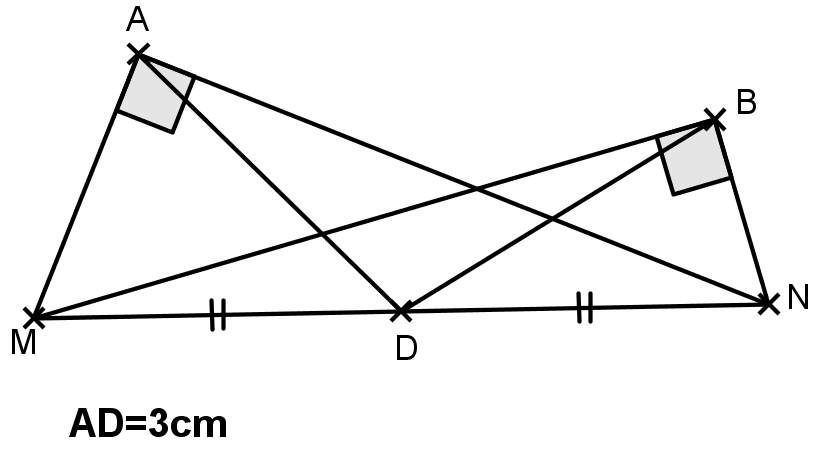
\includegraphics[width=6cm]{images/ex2.png} 
\end{center}


\subsection*{Exercice 3}


\begin{tabular}{cc}
\begin{minipage}{9cm}
Justifier chacune des affirmations suivantes:

\begin{enumerate}
  \item Le point E est le centre du cercle circonscrit au triangle VIC.
  \item Le point I appartient au cercle de diam�tre [CO].
\end{enumerate}

\end{minipage}
&
\begin{minipage}{9cm}
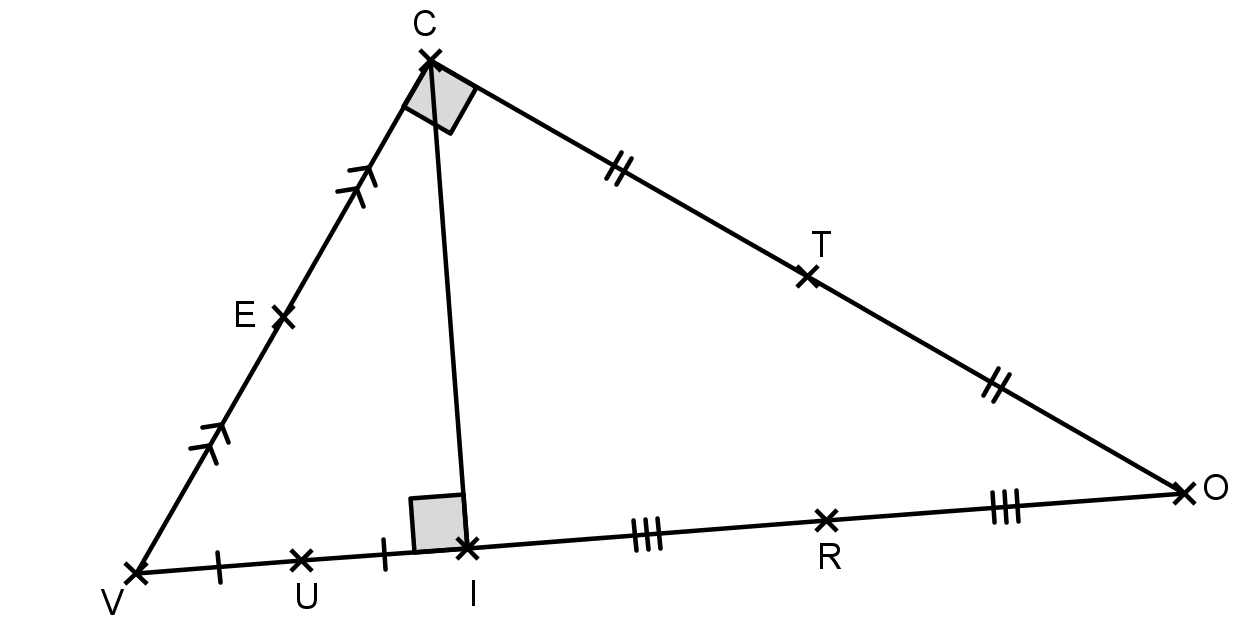
\includegraphics[width=9cm]{images/ex3.png}
\end{minipage}
\end{tabular}


\subsection*{Exercice 4}

Faire le n�13 p 145 de votre livre (constructions des triangles ONM et
EPK et justifications obligatoires, \textbf{le triangle ABC est facultatif et
sera not� hors bar�me}.)

\enskip

\fbox{
\begin{minipage}{18cm}
Cet exercice est un exercice de recherche. Les diff�rentes id�es, d�marches et
r�flexions seront �valu�es m�me si elles n'aboutissent pas.
\end{minipage}

}


\pagebreak


\section*{\center{Devoir maison 2}}

\textit{Devoir � rendre sur feuille grand format petits
carreaux pour le \ul{lundi 23 novembre 2009}.}

\enskip


\textit{Remarque: Chaque r�ponse doit �tre justifi�e par une propri�t� du cours. On
rappelle que voir ou mesurer � l'aide des instruments de g�om�trie n'est pas
une preuve.}

\subsection*{Exercice 1}

\begin{tabular}{cc}
\begin{minipage}{8cm}
\begin{enumerate}
  \item Calculer la mesure de l'angle $\widehat{POM}$? \\Justifier la r�ponse.
  \item Le point $O$ appartient-il au cercle de diam�tre $[PM]$?
\end{enumerate}
\end{minipage}
&
\begin{minipage}{9cm}
\begin{center}
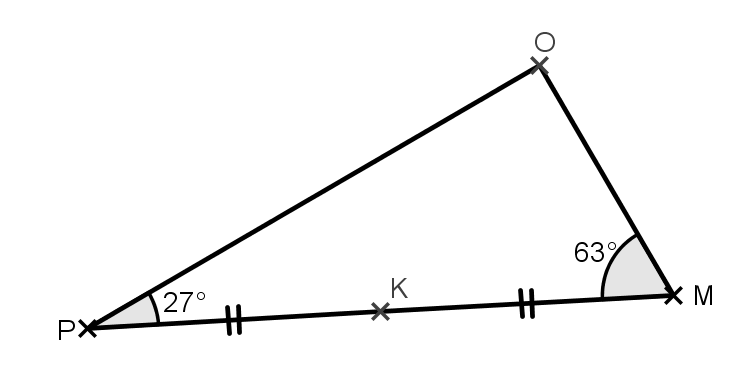
\includegraphics[width=7cm]{images/ex1bis.png}
\end{center}

\end{minipage}
\end{tabular}


\subsection*{Exercice 2}

\begin{tabular}{cc}
\begin{minipage}{9cm}

En utilisant les informations port�es sur la figure:


\begin{enumerate}
  \item Calculer MN.
  \item En d�duire BC.
\end{enumerate} 
\end{minipage}
&
\begin{minipage}{9cm}
\begin{center}
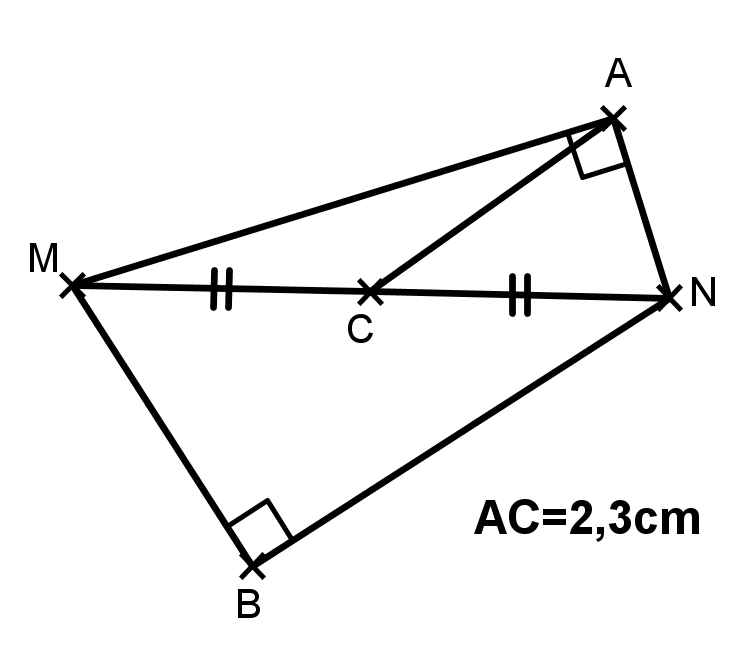
\includegraphics[width=5cm]{images/ex2bis.png}
\end{center}

\end{minipage}
\end{tabular}

\subsection*{Exercice 3}

\begin{tabular}{cc}
\begin{minipage}{9cm}
$E$ est le centre du cercle $\mathcal{M}$ et $G$ est le centre du cercle $\mathcal{N}$ .
\begin{enumerate}
  \item Montrer que le triangle $ACB$ est rectangle. Justifier.
  \item D�montrer que les droites $(ED)$ et $(DF)$ sont perpendiculaires.
\end{enumerate} 
\end{minipage}
&
\begin{minipage}{9cm}

\begin{center}
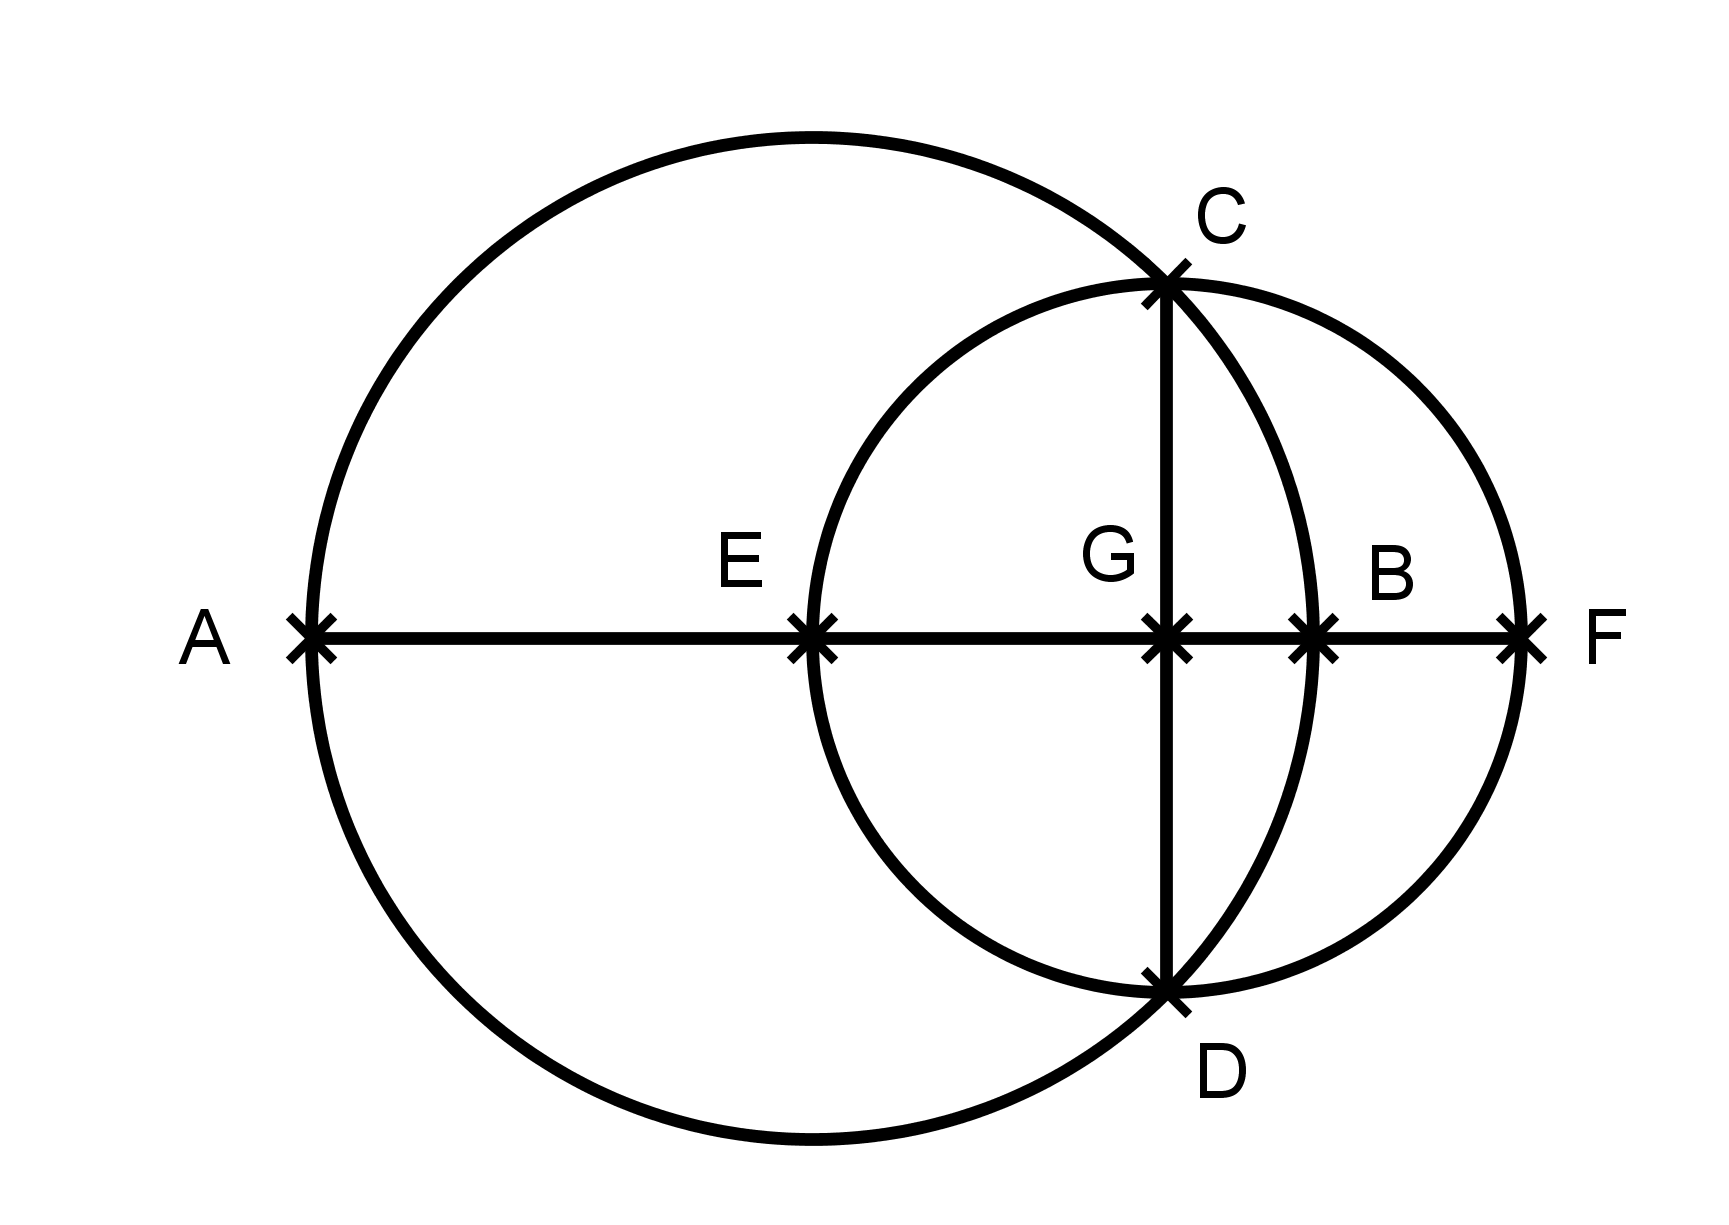
\includegraphics[width=6cm]{images/exo3bis.png}
\end{center}

\end{minipage}
\end{tabular}


\subsection*{Exercice 4}
\begin{tabular}{cc}
\begin{minipage}{8cm}
Pour chacun des triangles suivants, calculer la longueur manquante.
On donnera la valeur exacte ou un arrondi au dixieme pr�s.
\end{minipage}
&
\begin{minipage}{9cm}
\begin{center}
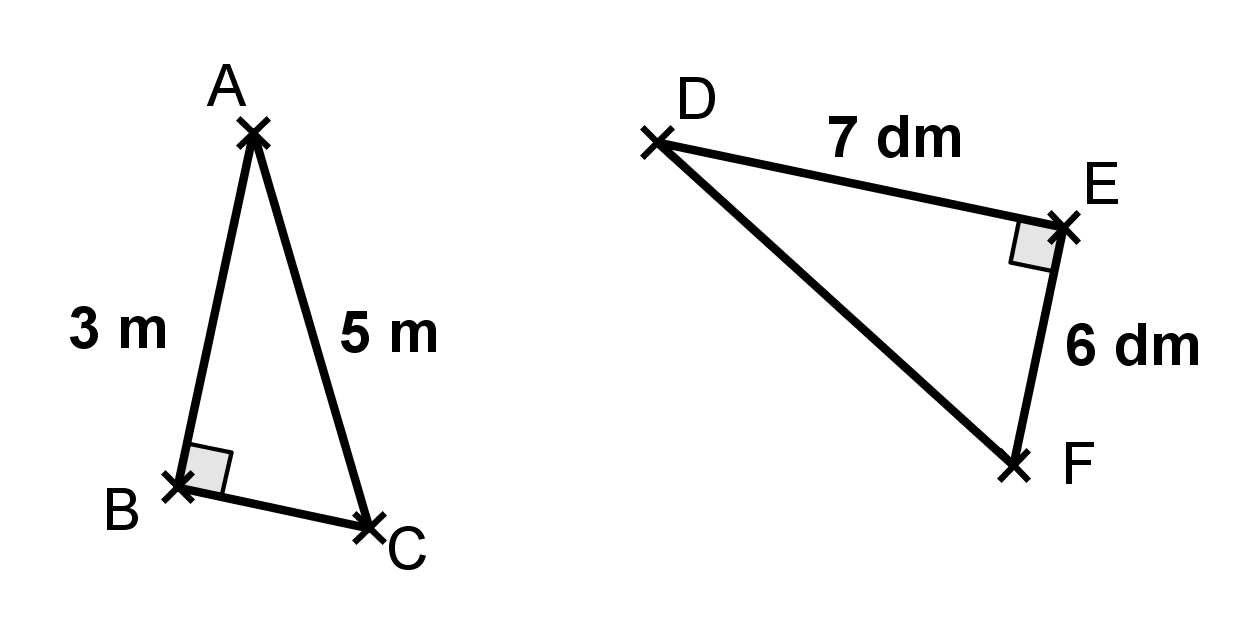
\includegraphics[width=7cm]{images/exo4.png}
\end{center}

\end{minipage} 
\end{tabular}
\end{document}
